\section[Lois de la dynamique du point]{Lois de la dynamique du point en référentiel non galiléen}

    \subsection{Les trois lois de Newton}

        \begin{enumerate}[label=\arabic*.]
            \item Principe d'inertie.
            \item La dérivée de la quantité de mouvement est égal à la somme des forces extérieures s'appliquant sur le système considéré dans un référentiel galiléen, c'est-à-dire
            \begin{equation*}
                \frac{\rmd\vec{p}}{\rmd t}=\vec{F^{\text{ext}}},\qquad \vec{p}=\gamma m\vec{v}\text{ dans }\mathcal{R}_{\text{galiléen}}.
            \end{equation*}
            \item Principe d'action-réaction.
        \end{enumerate}
        On se place dans le cadre classique ou $\gamma=1$.
    
    \subsection{Lois de la dynamique en référentiel non galiléen. Forces d'inertie}
        \subsubsection{Loi de la quantité de mouvement}

            On considère un référentiel $\mathcal{R}'$ en mouvement accéléré par rapport à un référentiel galiléen $\mathcal{R}_{\text{galiléen}}\equiv\mathcal{R}$. Dans $\mathcal{R}$, on a 
            \begin{align*}
                \frac{\rmd\vec{p}}{\rmd t}
                &=
                m\vec{a}(M)=\vec{F},\\
                &=m(\vec{a'}(M)+\vec{a_e}(M)+\vec{a_c}(M))=\vec{F}.
            \end{align*}
            On obtient ainsi
            \begin{equation*}
                m\vec{a'}(M)=\vec{F}+\vec{F_e}+\vec{F_c},
            \end{equation*}
            où $\vec{F_e}=-m\vec{a_e}$ et $\vec{F_e}=-m\vec{a_e}$. Ce sont des \og pseudo\fg~forces d'inertie.

        \subsubsection{Loi du moment cinétique par rapport à $O'$ fixe dans $\mathcal{R}'$ non galiléen.}

            Dans $\mathcal{R}'$, on a
            \begin{equation*}
                \left(\vec{L}_{O'}\right)_{\mathcal{R}'}\coloneqq\vec{O'M}\wedge\vec{p'}=\vec{O'M}\wedge m\vec{v'}(M).
            \end{equation*}
            Ainsi,
            \begin{align*}
                \left(\frac{\rmd \vec{L}_{O'}}{\rmd t}\right)
                &=
                m\underbrace{\left(\frac{\rmd \vec{O'M}}{\rmd t}\right)_{\mathcal{R}'}}_{\vec{v'}}\wedge\,\vec{v'}+\vec{O'M}\wedge\left(\frac{\rmd\vec{p}}{\rmd t}\right)_{\mathcal{R}'},\\
                &=\underbrace{\vec{O'M}\wedge \vec{F}}_{\vec{\mathcal{M}}_{O'}}+\underbrace{\vec{O'M}\wedge\vec{F_e}}_{\vec{\mathcal{M}}^{\text{ent}}_{O'}}+\underbrace{\vec{O'M}\wedge\vec{F_c}}_{\vec{\mathcal{M}}^{\text{coriolis}}_{O'}}.
            \end{align*}

        \subsubsection{Loi de l'énergie cinétique dans un référentiel non galiléen}
            
            \paragraph{Puissance des forces de Coriolis.}
                On a 
                \begin{equation*}
                    \vec{P}_{\text{cor}}=\vec{F_e}\cdot\vec{v'}=-m\left(2\vec{\omega}\wedge\vec{v'}\right)\wedge\vec{v'}=0.
                \end{equation*}
            
            \paragraph{Loi de l'énergie cinétique dans $\mathcal{R}'$.}
                On a 
                \begin{align*}
                    \frac{\rmd E_{c}'}{\rmd t} 
                    &= \frac{\rmd}{\rmd t}\left(\frac{1}{2}m v'^{2}\right),\\
                    &= m\vec{v}\cdot\left(\frac{\rmd\vec{v'}}{\rmd t}\right)_{\mathcal{R}'},\\
                    &=\left(\vec{F}+\vec{F_e}+\vec{F_c}\right)\cdot\vec{v'},\\
                    &=\left(\vec{F}+\vec{F_e}\right)\cdot\vec{v'},\\
                    &=P' + P_e'.
                \end{align*}
                Ainsi, on a 
                \begin{equation*}
                    \rmd E_c'=P'\rmd t+P_e'\rmd t=\vec{F}\cdot\underbrace{\vec{v'}\rmd t}_{\vec{\rmd l'}}+\vec{F_e}\cdot\underbrace{\vec{v'}_e\rmd t}_{\vec{\rmd l'}}=\delta W'+\delta W_e'.
                \end{equation*}
                En intégrant, on obtient donc
                \begin{equation*}
                    \boxed{\Delta E_c'=W'+W_e'.}    
                \end{equation*}
            
            \paragraph{Formulation en terme d'énergie mécanique.} Dans le cas où il existe des forces conservatives, on a $W_{\text{cons}}=-\Delta E_p$ (ou $\delta W_{\text{cons}}=-\rmd E_p$). Dans ce cas, on définit l'énergie mécanique par
            \begin{equation*}
                \boxed{E_m\coloneqq E_c+E_p.}
            \end{equation*}

            Ainsi, $\rmd E_c'=\delta W_{\text{nc}}-\rmd E_p'+\delta W_e'$ où $W_{\text{nc}}$ représente le travail venant de forces non conservatives. Alors 
            \begin{equation*}
                \rmd E_m'=\delta W_{\text{nc}}'+\delta W_{e}',
            \end{equation*}
            et on a donc
            \begin{equation*}
                \boxed{\Delta E_m'=W_{\text{nc}}'+W_e'.}
            \end{equation*}
        
    \subsection[Référentiel entraîné en translation accélérée]{Référentiel entraîné en translation accélérée}

        On a $\vec{F_e}=-m\vec{a}(O')$, force indépendante du point matériel $M$ considéré, et $\vec{F_c}=\vec{0}$.

        \subsubsection{Freinage d'une voiture}

            On suppose que la voiture roule initialement à 50 km/h et qu'elle s'arrête en 1 seconde. Alors
            \begin{equation*}
                \begin{aligned}
                    \left\lVert\vec{a_e}\right\rVert&\approx\frac{\Delta v}{\Delta t}=14~m.s^{-2}>g,\\
                    \left\lVert\vec{F_e}\right\rVert&=m\left\lVert \vec{a_e}\right\rVert=1400~N.
                \end{aligned}
            \end{equation*}

        \subsubsection{Pendule secoué}

            \begin{figure}
                \centering
                \tikzsetnextfilename{pendule_secoue}
                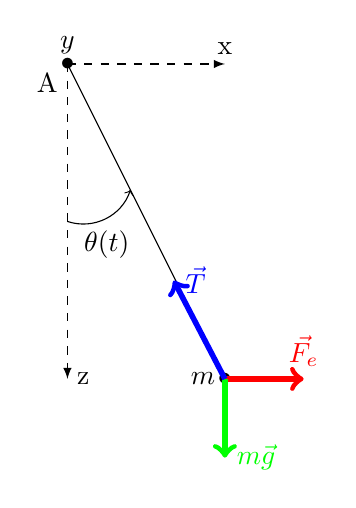
\begin{tikzpicture}
                    [scale=1,xscale=1,yscale=1]
                    
                    %\helpgrid{4}{4};
                    \coordinate (A) at (0,2); \coordinate (M) at (2,-2); \node at (A) {$\bullet$}; \node at (A) [below left] {A}; \node at (M) [left] {$m$}; \node at (M) {$\bullet$}; 
                    \node at (A) [above] {$y$};
                    
                    % Axe Oz
                    \draw [->,-latex,dashed] (0,2)--++(0,-4) node [right] {z}; 
                    
                    % Axe Ox
                    \draw [->,-latex,dashed] (0,2)--++(2,0) node [above] {x}; 
                    
                    % Axe Ox'
                    \draw (M) -- (0,2); \draw [->] (0,0) to [bend right=45] (0.8,0.4); \node at (0.5,-0.3) {$\theta(t)$}; 

                    % Forces
                    \draw [red, ->, line width=2pt] (M) -- (3,-2) node [above] {$\vec{F_e}$};
                    \draw [green, ->, line width=2pt] (M) -- (2,-3) node [right] {$m\vec{g}$};
                    \draw [blue, ->, line width=2pt] (M) -- (1.35,-0.75) node [right] {$\vec{T}$};
                \end{tikzpicture}
                \caption{Pendule secoué.}
                \label{fig:pendule_secoue}
            \end{figure}
            
            On considère un pendule secoué, voir la Figure~\ref{fig:pendule_secoue}. Le référentiel est $\mathcal{R}'=(Axyz)$ ($y$ est orienté vers nous). On suppose que le pendule situé en $A$ est secoué selon l'axe x : $x_{a}(t)=\alpha\cos(\omega t)$. Le théorème du moment cinétique par rapport à $A$ dans $\mathcal{R}'$ donne 
            \begin{equation*}
                \vec{L'_{A}}=J\dot{\theta}\vec{u_y}=ml^{2}\dot{\theta}\vec{u_y},
            \end{equation*}
            où $J$ est le moment d'inertie. On calcule la force d'entraînement :
            \begin{equation*}
                \left\lbrace
                \begin{aligned}
                    \vec{a_e} &=\ddot{x_A}(t)\vec{u_x}=-\omega^{2}\alpha\cos(\omega t)\vec{u_x},\\
                    \vec{F_e} &= m\omega^{2}\alpha\cos(\omega t)\vec{u_x}.
                \end{aligned}
                \right.
            \end{equation*}
            Le théorème du moment cinétique selon $\vec{u_y}$ donne alors
            \begin{equation*}
                ml^{2}\ddot{\theta}=-mgl\sin\theta+m\omega^{2}\alpha\cos(\omega t)l\cos\theta.
            \end{equation*}
            En notant $\omega_{0}^{2}=\dfrac{g}{l}$, on a donc 
            \begin{equation*}
                \boxed{
                    \ddot{\theta}+\omega_{0}^{2}\sin\theta=\frac{\omega^{2}\alpha}{l}\cos(\omega t)\cos\theta.
                }
            \end{equation*}

            Pour des petits mouvements, on a $\left\lvert\theta\right\rvert\ll1$ et on linéarise :
            \begin{equation*}
                \ddot{\theta}+\omega_{0}^{2}\theta=\frac{\omega^{2}\alpha}{l}\cos(\omega t).
            \end{equation*}
            En régime sinusoïdal forcé, $\ubar{\theta}(t)\propto\rme^{\rmj \omega t}$ (où $\rmj$ est le nombre imaginaire tel que $\rmj^{2}=-1$). Ainsi,
            \begin{equation*}
                \left(\omega_{0}^{2}-\omega^{2}\right)\ubar{\theta}(t)=\frac{\omega^{2}\alpha}{l}\rme^{\rmj\omega t}.
            \end{equation*}
            En prenant la partie réelle, on obtient donc
            \begin{equation*}
                \boxed{
                    \theta(t)=\frac{\omega^{2}}{\omega_{0}^{2}-\omega^{2}}\frac{\alpha}{l}\cos(\omega t).
                }
            \end{equation*}

            Si l'on suppose que le pendule est secoué selon l'axe z avec $z_{A}(t)=\alpha\cos(\omega t)$, on trouve pour équation du mouvement
            \begin{equation*}
                \ddot{\theta}+\omega_{0}^{2}\left(1+\frac{\alpha\omega^{2}}{g}\cos(\omega t)\right)\sin\theta = 0.
            \end{equation*}
            En posant $\Omega^{2}(t)=1+\dfrac{\alpha\omega^{2}}{g}\cos(\omega t)$, on voit qu'il s'agit d'un oscillateur paramétrique.

        \subsubsection{Énergie potentielle d'entraînement par translation uniformément accélérée}
            
            On a $\vec{a_e}=a\vec{u}_x$ et $\vec{F_e}=-ma\vec{u}_x$. Soit un déplacement élémentaire $\vec{\rmd l'}=\begin{pmatrix}\rmd x'\\\rmd y'\\\rmd z'\end{pmatrix} $ dans $\mathcal{R}'$. Alors 
            \begin{equation*}
                \delta W_e'=\vec{F_e}\cdot\vec{\rmd l'}=-ma\rmd x'=-\rmd(max')=-\rmd E_p^{\text{ent}}.
            \end{equation*}
            Ainsi, l'énergie potentielle d'entraînement vaut $E_{p}^{\text{ent}}=max'$ (à une constante près).

            \begin{example}
                \begin{figure}
                    \centering
                    \tikzsetnextfilename{pendule_train}
                    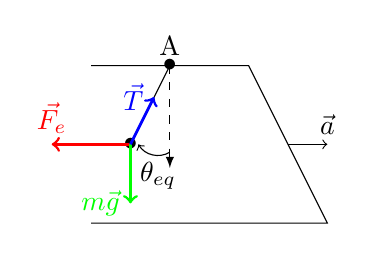
\begin{tikzpicture}
                        [scale=1,xscale=1,yscale=1]
                        
                        %\helpgrid{4}{4};
                        \coordinate (A) at (0,0); \coordinate (B) at (2,0); \coordinate (C) at (3,-2); \coordinate (D) at (0,-2);
                        \draw (A) -- (B) -- (C) -- (D);
                        \draw [->] (2.5,-1) -- (3,-1) node [above] {$\vec{a}$};

                        \coordinate (O) at (1,0); 
                        \node at (O) {$\bullet$}; \node at (O) [above] {A};

                        \draw [->,-latex,dashed] (O)--++(0,-1.3);
                        \coordinate (M) at (0.5,-1);
                        \node at (M) {$\bullet$};
                        \draw (M) -- (O); \draw [->] (1,-1.1) to [bend left=45] (0.6,-1); \node at (0.85,-1.4) {$\theta_{\text{eq}}$};
    
                        % Forces
                        \draw [red, ->, line width=1pt] (M) -- (-0.5,-1) node [above] {$\vec{F_e}$};
                        \draw [green, ->, line width=1pt] (M) -- (0.5,-1.75) node [left] {$m\vec{g}$};
                        \draw [blue, ->, line width=1pt] (M) -- (0.8,-0.4) node [left] {$\vec{T}$};
                    \end{tikzpicture}
                    \caption{Pendule dans un train en accélération uniforme.}    
                    \label{fig:pendule_train}
                \end{figure}
                On considère un pendule dans un train, voir la Figure~\ref{fig:pendule_train}. On cherche la valeur de $\theta_{\text{eq}}$.
                \begin{itemize}
                    \item \underline{Première méthode} : on utilise $\vec{\mathcal{M}_{A}^{\text{tot}}}=\vec{0}$. En projetant, on trouve alors $mgl\sin\theta_{\text{eq}}=mal\cos\theta_{\text{eq}}$ d'où 
                    \begin{equation*}
                        \tan\theta_{\text{eq}}=\frac{a}{g}.    
                    \end{equation*}
                    \item \underline{Deuxième méthode} : On a $E_p^{\text{ent}}=-mal\sin\theta$ et $E_p^{\text{poids}}=-mgl\cos\theta$ (avec éventuellement des constantes). Alors 
                    \begin{equation*}
                        \frac{\rmd E_p^{\text{tot}}}{\rmd\theta}=0=-mal\cos\theta+mgl\sin\theta,
                    \end{equation*}
                    d'où le résultat.
                \end{itemize}
            \end{example}
    
    \subsection[Référentiel entraîné en rotation uniforme]{Référentiel entraîné en rotation uniforme par\\rapport à un axe fixe}

        On suppose que la rotation se fait selon l'axe $(Oz)$ à une vitesse angulaire $\omega$, voir la Figure~\ref{fig:rotation_uniforme}. $H$ est le projeté du point $M$ sur l'axe $(Oz)$. On a $\vec{F_e}=-2m\vec{\omega}\wedge\vec{v}$, qui est donc perpendiculaire au mouvement dans $\mathcal{R}'$.

        \begin{figure}
            \centering
            \tikzsetnextfilename{axe_rotation_uniforme}
            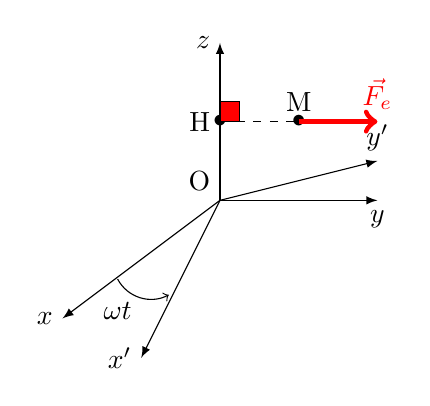
\begin{tikzpicture}[scale=1]  
                % \helpgrid{3}{3}
            \draw [->,-latex] (0,0) --++ (-1,-2) node [left] {$x'$}	;   
            \draw [->,-latex] (0,0) --++ (2,0) node [below] {$y$}	;
            \draw [->,-latex] (0,0) --++ (0,2) node [left] {$z$}	; 

            \draw [->,-latex] (0,0) --++ (-2,-1.5) node [left] {$x$}	; 
            \draw [->,-latex] (0,0) --++ (2,0.5) node [above] {$y'$}	; 
            \coordinate (H) at (0,1); \node at (H) {$\bullet$};
            \node at (H) [left] {H};
            \coordinate (O) at (0,0); \node at (O) [above left] {O};                      
            \coordinate (M) at (1,1); \node at (M) {$\bullet$}; \node at (M) [above] {M};
            \draw [red, ->, line width=2pt] (M) -- (2,1) node [above] {$\vec{F_e}$};
            \draw [dashed] (H) -- (M); 
            \draw [fill=red](H) rectangle ++(0.25,0.25);

            \draw [->] (-1.3,-1) to [bend right=45] (-0.65,-1.2); \node at (-1.3,-1.4) {$\omega t$}; 
            \end{tikzpicture}
            \caption{Rotation uniforme autour de l'axe $(Oz)$.}    
            \label{fig:rotation_uniforme}
        \end{figure}

        \subsubsection{Exemple}

            On considère le cas où l'on rajoute un ressort sur l'axe $(Ox')$, fixé en $O$, de constante de raideur $k$ et de longueur au repos $l_0$, avec au bout une masse $m$, voir la Figure~\ref{fig:exemple_rotation_uniforme}.           

            \begin{figure}
                \centering
                \tikzsetnextfilename{exemple_axe_rotation_uniforme}
                \begin{tikzpicture}[scale=1]  
                    % \helpgrid{3}{3}
                \draw [->,-latex] (0,0) --++ (-1,-2) node [left] {$x'$}	;   
                \draw [->,-latex] (0,0) --++ (2,0) node [below] {$y$}	;
                \draw [->,-latex] (0,0) --++ (0,2) node [left] {$z$}	; 
    
                \draw [->,-latex] (0,0) --++ (-2,-1.5) node [left] {$x$}	; 
                \draw [->,-latex] (0,0) --++ (2,0.5) node [above] {$y'$}	; 
                \coordinate (O) at (0,0); \node at (O) [above left] {O};                      
    
                \draw [->] (-1.3,-1) to [bend right=45] (-0.75,-1.3); \node at (-1.3,-1.4) {$\omega t$}; 
                \draw [ressort,decorate,decoration={coil,aspect=0.3,segment length=1.5mm,amplitude=3mm}] (O)--++(-0.65,-1.3);
                \node at (-0.65,-1.3) {$\bullet$}; \node at (-0.65,-1.3) [below right] {$m$};
                \node at (0.3, -0.7) {$k$};
                \end{tikzpicture}
                \caption{Exemple de rotation uniforme autour de l'axe $(Oz)$ : ressort avec une masse.}    
                \label{fig:exemple_rotation_uniforme}
            \end{figure}
            
            On cherche l'expression de $x'(t)$. On a
            \begin{equation*}
                \left\lbrace
                \begin{aligned}
                    \vec{F_e} &= m\omega^{2}x'(t)\vec{u_{x'}},\\
                    \vec{F_c} &= -2m\omega\vec{u_z}\wedge \dot{x'}(t)\vec{u_{x'}}=-2m\omega\dot{x'}(t)\vec{u_y}.
                \end{aligned}
                \right.
            \end{equation*}
            On projette le principe fondamental de la dynamique selon $\vec{u_x'}$ pour obtenir
            \begin{equation*}
                m\ddot{x'}(t)=-k\left(x'(t)-l_0\right)+m\omega^{2}x'(t).
            \end{equation*}
            En posant $\omega_{0}^{2}\coloneqq\frac{k}{m}$, on obtient 
            \begin{equation*}
                \ddot{x'}(t)+\left(\omega_{0}^{2}-\omega^{2}\right)x'(t)=\omega_{0}^{2}l_0.
            \end{equation*}

        \subsubsection{Énergie potentielle d'entraînement \og centrifuge\fg}
            
            Soit un déplacement $\vec{dl'}=dx'\vec{u_{x'}}$ dans $\mathcal{R}'$. On a 
            \begin{equation*}
                \delta W_{e}'=\vec{F_e}\cdot\vec{dl'}=m\omega^{2}x'\rmd x'=\rmd\left(m\omega^{2}\frac{x'^{2}}{2}\right)\coloneqq -\rmd E_p^{\text{ent}},
            \end{equation*}
            d'où $E_p^{\text{ent}}=-m\omega^{2}\frac{x'^{2}}{2}$.

        \subsubsection{Retour sur l'exemple}

            On applique le théorème d'énergie mécanique dans $\mathcal{R}'$ :
            \begin{equation*}
                E_{m_{tot}}'=\text{constante}=\frac{1}{2}m\dot{x'}^{2}+\frac{1}{2}k(x'-l_0)^{2}-m\omega^{2}\frac{x'^{2}}{2}.
            \end{equation*}

            On se donne comme conditions initiales $x'(0)=l_0$ et $\dot{x'}(0)=0$. On a alors 
            \begin{equation*}
                \boxed{
                    \frac{1}{2}m\dot{x'}^{2}+\frac{1}{2}k(x'-l_0)^{2}-\frac{m\omega^{2}x'^{2}}{2}=-\frac{m\omega^{2}l_0^{2}}{2}.
                }
            \end{equation*}
